\documentclass{boi2014-et}

\usepackage{tikz}

\renewcommand{\DayNum}{2}
\renewcommand{\TaskCode}{demarcation}
\renewcommand{\TaskName}{Piiri tõmbamine}

\newcommand{\constant}[1]{{\tt #1}}

\begin{document}

    \begin{wrapfigure}{r}{3cm}
        \vspace{-24pt}
        \includegraphics[width=3cm]{\TaskCode.jpeg}
    \end{wrapfigure}

    Kaua aega valitses Bytopia saart hea kuningas Byteasar.
    Pärast kuninga ootamatut surma ei suutnud tema kaksikud pojad
    Biteon ja Byteon otsustada, kumb neist peaks troonile asuma.
    Seetõttu otsustati jagada saar kaheks provintsiks ja neid
    sõltumatult valitseda.

    Kaardil on Byteotia $N$ tipuga hulknurga kujuline.
    Hulknurga kõik servad on paralleelsed ristkülikukujulise kaardi külgedega ning
    iga kaks järjestikust serva paiknevad teineteise suhtes täisnurga all.
    Hulknurga ükski serv ei lõika ega puutu ühtki teist serva välja arvatud
    järjestikused servad nende ühises otspunktis.

    Biteon ja Byteon tahavad jagada hulknurga kaheks kongruentseks hulknurgaks,
    kasutades poolitamiseks üht sirglõiku,
    mis on hulknurga sees ning paralleelne ühega kaardi külgedest.
    (Kaks kujundit on kongruentsed, kui üht saab muuta teiseks,
    kasutades peegeldusi, pööramisi ja nihutamisi.)
    Hulknurga tippude koordinaadid ja jagamiseks
    kasutatava sirglõigu otspunktide koordinaadid on täisarvud.

    Kuningapojad küsivad, kas selline jagamine on võimalik.

    \Task

    Leida saare kuju põhjal, kas seda saab horisontaalse või vertikaalse sirglõiguga
    kaheks kongruentseks hulknurgaks jagada.
    Kui saab, siis leida selline lõik.

    \Input

    Sisendi esimesel real on tippude arv $N$.
    Järgmisel $N$ real on igaühel tühikuga eraldatud täisarvude paar
    $X_i$ ja $Y_i$ ($0 \le X_i, Y_i \le 10^9$), $i$. tipu koordinaadid.

    Tipud on antud järjekorras, s.t lõigud $(X_1,Y_1) - (X_2,Y_2)$,
    $(X_2,Y_2) - (X_3,Y_3)$, \ldots, $(X_{N-1},Y_{N-1}) - (X_N,Y_N)$ ja
    $(X_N,Y_N) - (X_1,Y_1)$ on parajasti hulknurga servad.
    Lisaks on teada, et iga kaks järjestikust serva on teineteisega risti.

    \Output

    Programm peab väljastama ühe rea.
    Kui saare jagamine on võimalik, väljastada 4 tühikutega eraldatud täisarvu
    $x_1$, $y_1$, $x_2$ ja $y_2$, mis tähistavad sirglõiku otspunktidega
    $(x_1, y_1)$ ja $(x_2, y_2)$.
    Peab kehtima kas $x_1 = x_2$ või $y_1 = y_2$.
    Lõik peab olema hulknurga sees ja ainult selle otspunktid võivad
    hulknurga piirjoont puutuda.

    Kui selline jagamine pole võimalik, väljastada sõna \constant{NO}.

\clearpage

    \Examples

    \example
    {
        10 \newline
        0 0 \newline
        1 0 \newline
        1 1 \newline
        3 1 \newline
        3 5 \newline
        2 5 \newline
        2 3 \newline
        1 3 \newline
        1 2 \newline
        0 2
    }
    {
        1 2 3 2
    }
    {
        {\tt 3 2 1 2} \newline
        oleks ka õige vastus.

        \begin{center}
            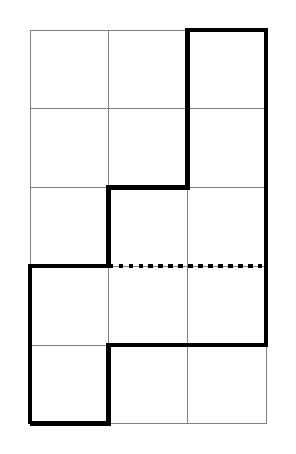
\begin{tikzpicture}
            \draw[help lines] (0,0) grid (3,5);
            \draw[ultra thick] (0,0) -- (1,0) -- (1,1) -- (3,1) -- (3,5) --
                         (2,5) -- (2,3) -- (1,3) -- (1,2) -- (0,2) -- (0,0);
            \draw[ultra thick,dotted] (1,2) -- (3,2);
            \end{tikzpicture}
        \end{center}
    }

    \example
    {
        6 \newline
        0 0 \newline
        1 0 \newline
        1 1 \newline
        2 1 \newline
        2 2 \newline
        0 2
    }
    {
        NO
    }
    {
        Selles näites ei saa saart kaheks kongruentseks osaks jagada.

        \begin{center}
            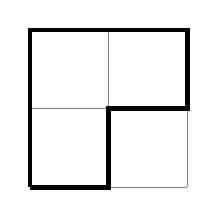
\begin{tikzpicture}
            \draw[help lines] (0,0) grid (2,2);
            \draw[ultra thick] (0,0) -- (1,0) -- (1,1) --
                         (2,1) -- (2,2) -- (0,2) -- (0,0);
            \end{tikzpicture}
        \end{center}
    }

    \Scoring

    \begin{description}
        \item[Alamülesanne 1 (12 punkti).] $4 \le N \le 100\,000$.
            Mistahes horisontaalne või vertikaalne joon, mis hulknurka lõikab,
            jagab selle täpselt kaheks osaks.
        \item[Alamülesanne 2 (15 punkti).] $4 \le N \le 200$.
        \item[Alamülesanne 3 (23 punkti).] $4 \le N \le 4\,000$.
        \item[Alamülesanne 4 (50 punkti).] $4 \le N \le 100\,000$.
    \end{description}

    \Constraints

    \begin{description}
        \item[Ajapiirang:] 0,5 s.
        \item[Mälupiirang:] 256 MB.
    \end{description}

\end{document}
